\documentclass[11pt]{article}\usepackage[]{graphicx}\usepackage[]{xcolor}
% maxwidth is the original width if it is less than linewidth
% otherwise use linewidth (to make sure the graphics do not exceed the margin)
\makeatletter
\def\maxwidth{ %
  \ifdim\Gin@nat@width>\linewidth
    \linewidth
  \else
    \Gin@nat@width
  \fi
}
\makeatother

\definecolor{fgcolor}{rgb}{0.345, 0.345, 0.345}
\newcommand{\hlnum}[1]{\textcolor[rgb]{0.686,0.059,0.569}{#1}}%
\newcommand{\hlsng}[1]{\textcolor[rgb]{0.192,0.494,0.8}{#1}}%
\newcommand{\hlcom}[1]{\textcolor[rgb]{0.678,0.584,0.686}{\textit{#1}}}%
\newcommand{\hlopt}[1]{\textcolor[rgb]{0,0,0}{#1}}%
\newcommand{\hldef}[1]{\textcolor[rgb]{0.345,0.345,0.345}{#1}}%
\newcommand{\hlkwa}[1]{\textcolor[rgb]{0.161,0.373,0.58}{\textbf{#1}}}%
\newcommand{\hlkwb}[1]{\textcolor[rgb]{0.69,0.353,0.396}{#1}}%
\newcommand{\hlkwc}[1]{\textcolor[rgb]{0.333,0.667,0.333}{#1}}%
\newcommand{\hlkwd}[1]{\textcolor[rgb]{0.737,0.353,0.396}{\textbf{#1}}}%
\let\hlipl\hlkwb

\usepackage{framed}
\makeatletter
\newenvironment{kframe}{%
 \def\at@end@of@kframe{}%
 \ifinner\ifhmode%
  \def\at@end@of@kframe{\end{minipage}}%
  \begin{minipage}{\columnwidth}%
 \fi\fi%
 \def\FrameCommand##1{\hskip\@totalleftmargin \hskip-\fboxsep
 \colorbox{shadecolor}{##1}\hskip-\fboxsep
     % There is no \\@totalrightmargin, so:
     \hskip-\linewidth \hskip-\@totalleftmargin \hskip\columnwidth}%
 \MakeFramed {\advance\hsize-\width
   \@totalleftmargin\z@ \linewidth\hsize
   \@setminipage}}%
 {\par\unskip\endMakeFramed%
 \at@end@of@kframe}
\makeatother

\definecolor{shadecolor}{rgb}{.97, .97, .97}
\definecolor{messagecolor}{rgb}{0, 0, 0}
\definecolor{warningcolor}{rgb}{1, 0, 1}
\definecolor{errorcolor}{rgb}{1, 0, 0}
\newenvironment{knitrout}{}{} % an empty environment to be redefined in TeX

\usepackage{alltt}
\usepackage[margin=2.3cm,headheight=14pt]{geometry}
\usepackage[T1]{fontenc}
\usepackage{lmodern}
\usepackage{amsmath,amssymb}
\usepackage{booktabs}
\usepackage{enumitem}
\usepackage{float}
\usepackage{fancyhdr}
\usepackage[hidelinks]{hyperref}

\renewcommand{\figurename}{Figura}
\renewcommand{\tablename}{Tabla}
\renewcommand{\contentsname}{Contenido}

\pagestyle{fancy}
\fancyhf{}
\lhead{MAT5519 Clasificación no Supervisada}
\rhead{C. G. Mayorga Tapia (00294506)}
\cfoot{\thepage}

\newcommand{\norm}[1]{\left\lVert #1 \right\rVert}
\setlength{\parindent}{0pt}
\setlength{\parskip}{6pt}
\IfFileExists{upquote.sty}{\usepackage{upquote}}{}
\begin{document}



\begin{center}
{\Large\bfseries Ejercicios de Análisis de Clusters}\\[4pt]
MAT5519 (10160) Clasificación no Supervisada\\
Septiembre--Diciembre 2026\\[10pt]
\textbf{Carlos Guillermo Mayorga Tapia}\\
ID: 00294506\\[4pt]
12 de noviembre de 2026
\end{center}

\vspace{6pt}
\hrule

%=====================================================================
\section{Distancias}
\subsection{Distancias y desigualdad triangular}

En todo el ejercicio uso $\norm{u}_q = \left(\sum_{i=1}^p |u_i|^q\right)^{1/q}$ y quiero ver que
\[
\norm{x-y}_q \le \norm{x-z}_q + \norm{z-y}_q .
\]

%---------------------------------------------------------------------
\subsubsection*{(a) Caso de una dimensión}

Quiero probar $|a-b| \le |a-c| + |c-b|$ para $a,b,c\in\mathbb{R}$.

\textbf{Simplificación.} Si intercambio $a$ y $b$, el lado izquierdo queda $|b-a| = |a-b|$ y el lado derecho queda $|b-c|+|c-a| = |c-b| + |a-c|$, que es lo mismo. Entonces basta revisar el caso $a \le b$, donde $|a-b| = b-a$.

Con $a\le b$, el punto $c$ solo puede estar en tres lugares:

\textbf{Caso 1: $c$ está entre $a$ y $b$, es decir $a \le c \le b$.}
\begin{align*}
a - c \le 0 &\;\Rightarrow\; |a-c| = c-a,\\
c - b \le 0 &\;\Rightarrow\; |c-b| = b-c,\\
|a-c| + |c-b| &= (c-a) + (b-c)\\
&= b - a\\
&= |a-b|.
\end{align*}
Aquí se cumple con igualdad.

\textbf{Caso 2: $c$ está a la izquierda, $c < a \le b$.}
\begin{align*}
a - c > 0 &\;\Rightarrow\; |a-c| = a-c,\\
c - b < 0 &\;\Rightarrow\; |c-b| = b-c,\\
|a-c| + |c-b| &= (a-c) + (b-c)\\
&= a + b - 2c\\
&= (b-a) + 2a - 2c\\
&= (b-a) + 2(a-c).
\end{align*}
Como $a - c > 0$, entonces $2(a-c) > 0$ y
\[
|a-c| + |c-b| = (b-a) + 2(a-c) > b-a = |a-b|.
\]

\textbf{Caso 3: $c$ está a la derecha, $a \le b < c$.}
\begin{align*}
a - c < 0 &\;\Rightarrow\; |a-c| = c-a,\\
c - b > 0 &\;\Rightarrow\; |c-b| = c-b,\\
|a-c| + |c-b| &= (c-a) + (c-b)\\
&= 2c - a - b\\
&= (b-a) + 2c - 2b\\
&= (b-a) + 2(c-b).
\end{align*}
Como $c - b > 0$, entonces $2(c-b)>0$ y
\[
|a-c| + |c-b| = (b-a) + 2(c-b) > b-a = |a-b|.
\]

En los tres casos $|a-b| \le |a-c| + |c-b|$. \hfill$\square$

\textbf{Consecuencia para $p=1$.} Si $p=1$, el vector $u$ es un solo número y
\[
\norm{u}_q = \left(|u|^q\right)^{1/q} = |u|^{q\cdot \frac{1}{q}} = |u|,
\]
lo cual vale para cualquier $q>0$ porque $|u|\ge 0$. Entonces
\[
\norm{x-y}_q = |x-y|,\qquad \norm{x-z}_q = |x-z|,\qquad \norm{z-y}_q = |z-y|,
\]
y la desigualdad (1.1) se vuelve exactamente (1.2) con $a=x$, $b=y$, $c=z$. Por lo tanto (1.1) se cumple en $p=1$ para toda $q>0$ (incluso para $q<1$).

%---------------------------------------------------------------------
\subsubsection*{(b) Caso $q=1$ (Manhattan)}

Para cada coordenada $i = 1,\dots,p$ uso (1.2) con $a=x_i$, $b=y_i$, $c=z_i$:
\[
|x_i - y_i| \le |x_i - z_i| + |z_i - y_i|, \qquad i = 1,\dots,p.
\]
Sumo las $p$ desigualdades (al sumar desigualdades del mismo sentido, el sentido se mantiene):
\begin{align*}
\norm{x-y}_1 &= \sum_{i=1}^p |x_i - y_i|\\
&\le \sum_{i=1}^p \big(|x_i - z_i| + |z_i - y_i|\big)\\
&= \sum_{i=1}^p |x_i - z_i| + \sum_{i=1}^p |z_i - y_i|\\
&= \norm{x-z}_1 + \norm{z-y}_1. \hspace{6cm}\square
\end{align*}

%---------------------------------------------------------------------
\subsubsection*{(c) Caso $q=2$ (euclidiana)}

Tomo $u = x - z$ y $v = z - y$. Entonces
\[
u + v = (x - z) + (z - y) = x - y,
\]
y lo que quiero probar es $\norm{u+v}_2 \le \norm{u}_2 + \norm{v}_2$. Trabajo con el cuadrado para quitar la raíz:
\begin{align*}
\norm{u+v}_2^2 &= \sum_{i=1}^p (u_i + v_i)^2\\
&= \sum_{i=1}^p \left(u_i^2 + 2u_iv_i + v_i^2\right)\\
&= \sum_{i=1}^p u_i^2 + 2\sum_{i=1}^p u_iv_i + \sum_{i=1}^p v_i^2\\
&= \norm{u}_2^2 + 2\sum_{i=1}^p u_iv_i + \norm{v}_2^2\\
&\le \norm{u}_2^2 + 2\norm{u}_2\norm{v}_2 + \norm{v}_2^2 \qquad \text{(Cauchy-Schwarz)}\\
&= \left(\norm{u}_2 + \norm{v}_2\right)^2.
\end{align*}
Los dos lados son no negativos y la raíz cuadrada es creciente en $[0,\infty)$, así que puedo sacar raíz sin cambiar el sentido:
\[
\norm{u+v}_2 \le \norm{u}_2 + \norm{v}_2
\quad\Longrightarrow\quad
\norm{x-y}_2 \le \norm{x-z}_2 + \norm{z-y}_2. \hspace{2cm}\square
\]

%---------------------------------------------------------------------
\subsubsection*{(d) Caso $q=\infty$ (máxima distancia)}

Fijo cualquier coordenada $i$. Por (1.2):
\[
|x_i - y_i| \le |x_i - z_i| + |z_i - y_i|.
\]
El máximo de una lista es mayor o igual que cualquier elemento de la lista, por eso
\[
|x_i - z_i| \le \max_{j} |x_j - z_j| = \norm{x-z}_\infty,
\qquad
|z_i - y_i| \le \max_{j} |z_j - y_j| = \norm{z-y}_\infty.
\]
Juntando:
\[
|x_i - y_i| \le \norm{x-z}_\infty + \norm{z-y}_\infty \qquad \text{para toda } i = 1,\dots,p.
\]
El lado derecho no depende de $i$, es una cota que sirve para todas las coordenadas. En particular sirve para la coordenada donde $|x_i - y_i|$ es más grande:
\[
\norm{x-y}_\infty = \max_{i} |x_i - y_i| \le \norm{x-z}_\infty + \norm{z-y}_\infty. \hspace{3cm}\square
\]

%---------------------------------------------------------------------
\subsubsection*{(e) Contraejemplo con $q = 1/2$ y $p = 2$}

Con $q = 1/2$:
\[
\norm{u}_{1/2} = \left(|u_1|^{1/2} + |u_2|^{1/2}\right)^{2} = \left(\sqrt{|u_1|} + \sqrt{|u_2|}\right)^{2}.
\]
Tomo los puntos
\[
x = (0,0), \qquad y = (1,1), \qquad z = (1,0).
\]

\textbf{Lado izquierdo.}
\[
x - y = (0-1,\;0-1) = (-1,-1),\qquad
\norm{x-y}_{1/2} = \left(\sqrt{1} + \sqrt{1}\right)^2 = (1+1)^2 = 2^2 = 4.
\]

\textbf{Lado derecho.}
\begin{align*}
x - z &= (0-1,\;0-0) = (-1,0), & \norm{x-z}_{1/2} &= \left(\sqrt{1} + \sqrt{0}\right)^2 = (1+0)^2 = 1,\\
z - y &= (1-1,\;0-1) = (0,-1), & \norm{z-y}_{1/2} &= \left(\sqrt{0} + \sqrt{1}\right)^2 = (0+1)^2 = 1.
\end{align*}
Entonces
\[
\norm{x-z}_{1/2} + \norm{z-y}_{1/2} = 1 + 1 = 2 .
\]
Para que se cumpliera la desigualdad necesitaría $4 \le 2$, lo cual es falso. Por lo tanto la desigualdad triangular no se cumple con $q=1/2$: ir de $x$ a $y$ ``directo'' sale más caro que pasar por $z$.

Lo confirmo rápido en R:

\begin{knitrout}\small
\definecolor{shadecolor}{rgb}{0.969, 0.969, 0.969}\color{fgcolor}\begin{kframe}
\begin{alltt}
\hldef{lq} \hlkwb{<-} \hlkwa{function}\hldef{(}\hlkwc{u}\hldef{,} \hlkwc{q}\hldef{)} \hlkwd{sum}\hldef{(}\hlkwd{abs}\hldef{(u)}\hlopt{^}\hldef{q)}\hlopt{^}\hldef{(}\hlnum{1}\hlopt{/}\hldef{q)}
\hldef{x} \hlkwb{<-} \hlkwd{c}\hldef{(}\hlnum{0}\hldef{,} \hlnum{0}\hldef{); y} \hlkwb{<-} \hlkwd{c}\hldef{(}\hlnum{1}\hldef{,} \hlnum{1}\hldef{); z} \hlkwb{<-} \hlkwd{c}\hldef{(}\hlnum{1}\hldef{,} \hlnum{0}\hldef{)}
\hlkwd{c}\hldef{(}\hlkwc{izq} \hldef{=} \hlkwd{lq}\hldef{(x} \hlopt{-} \hldef{y,} \hlnum{1}\hlopt{/}\hlnum{2}\hldef{),} \hlkwc{der} \hldef{=} \hlkwd{lq}\hldef{(x} \hlopt{-} \hldef{z,} \hlnum{1}\hlopt{/}\hlnum{2}\hldef{)} \hlopt{+} \hlkwd{lq}\hldef{(z} \hlopt{-} \hldef{y,} \hlnum{1}\hlopt{/}\hlnum{2}\hldef{))}
\end{alltt}
\begin{verbatim}
izq der 
  4   2 
\end{verbatim}
\end{kframe}
\end{knitrout}

%=====================================================================
\section{Análisis de Clusters}
\subsection{Análisis de clustering jerárquico}

Numero las filas de $X$ como puntos:
\[
P_1 = (-1,1),\quad P_2 = (-1,-1),\quad P_3 = (0,0),\quad P_4 = (1.3,0),\quad P_5 = (2.3,0).
\]
Uso $d(P_r,P_s) = \sqrt{(x_{r1}-x_{s1})^2 + (x_{r2}-x_{s2})^2}$ y redondeo a 3 decimales, que es suficiente para comparar.

%---------------------------------------------------------------------
\subsubsection*{(a) Matriz de distancias euclidianas}

\begin{align*}
d_{12} &= \sqrt{(-1-(-1))^2 + (1-(-1))^2} = \sqrt{0^2 + 2^2} = \sqrt{4} = 2.000\\
d_{13} &= \sqrt{(-1-0)^2 + (1-0)^2} = \sqrt{1 + 1} = \sqrt{2} \approx 1.414\\
d_{14} &= \sqrt{(-1-1.3)^2 + (1-0)^2} = \sqrt{(-2.3)^2 + 1^2} = \sqrt{5.29 + 1} = \sqrt{6.29} \approx 2.508\\
d_{15} &= \sqrt{(-1-2.3)^2 + (1-0)^2} = \sqrt{(-3.3)^2 + 1^2} = \sqrt{10.89 + 1} = \sqrt{11.89} \approx 3.448\\
d_{23} &= \sqrt{(-1-0)^2 + (-1-0)^2} = \sqrt{1 + 1} = \sqrt{2} \approx 1.414\\
d_{24} &= \sqrt{(-1-1.3)^2 + (-1-0)^2} = \sqrt{5.29 + 1} = \sqrt{6.29} \approx 2.508\\
d_{25} &= \sqrt{(-1-2.3)^2 + (-1-0)^2} = \sqrt{10.89 + 1} = \sqrt{11.89} \approx 3.448\\
d_{34} &= \sqrt{(0-1.3)^2 + (0-0)^2} = \sqrt{1.69} = 1.300\\
d_{35} &= \sqrt{(0-2.3)^2 + (0-0)^2} = \sqrt{5.29} = 2.300\\
d_{45} &= \sqrt{(1.3-2.3)^2 + (0-0)^2} = \sqrt{1} = 1.000
\end{align*}

La matriz es simétrica con ceros en la diagonal, así que solo escribo la parte de abajo:
\[
D = \begin{array}{c|ccccc}
 & P_1 & P_2 & P_3 & P_4 & P_5\\ \hline
P_1 & 0 & & & & \\
P_2 & 2.000 & 0 & & & \\
P_3 & 1.414 & 1.414 & 0 & & \\
P_4 & 2.508 & 2.508 & 1.300 & 0 & \\
P_5 & 3.448 & 3.448 & 2.300 & 1.000 & 0
\end{array}
\]

Algo que se ve desde aquí: $P_1$ y $P_2$ son espejo uno del otro respecto al eje horizontal, por eso $d_{13}=d_{23}$, $d_{14}=d_{24}$ y $d_{15}=d_{25}$.

%---------------------------------------------------------------------
\subsubsection*{(b) Clustering jerárquico}

En cada paso uno el par de grupos más cercano y actualizo las distancias del grupo nuevo $A\cup B$ contra cualquier otro grupo $C$ con:
\[
\text{Simple: } d(A\cup B, C) = \min\{d(A,C),\, d(B,C)\},
\qquad
\text{Completo: } d(A\cup B, C) = \max\{d(A,C),\, d(B,C)\}.
\]

\paragraph{Aglomeramiento simple.}

\textbf{Paso 1.} El mínimo de $D$ es $d_{45} = 1.000$. Uno $\{P_4,P_5\}$ a altura $1.000$. Actualizo:
\begin{align*}
d(\{4,5\}, 1) &= \min\{d_{14}, d_{15}\} = \min\{2.508,\, 3.448\} = 2.508\\
d(\{4,5\}, 2) &= \min\{d_{24}, d_{25}\} = \min\{2.508,\, 3.448\} = 2.508\\
d(\{4,5\}, 3) &= \min\{d_{34}, d_{35}\} = \min\{1.300,\, 2.300\} = 1.300
\end{align*}
\[
\begin{array}{c|cccc}
 & P_1 & P_2 & P_3 & \{4,5\}\\ \hline
P_1 & 0 & & & \\
P_2 & 2.000 & 0 & & \\
P_3 & 1.414 & 1.414 & 0 & \\
\{4,5\} & 2.508 & 2.508 & \mathbf{1.300} & 0
\end{array}
\]

\textbf{Paso 2.} El mínimo es $1.300$ entre $P_3$ y $\{4,5\}$. Uno $\{P_3,P_4,P_5\}$ a altura $1.300$. Actualizo:
\begin{align*}
d(\{3,4,5\}, 1) &= \min\{d_{13},\, d(\{4,5\},1)\} = \min\{1.414,\, 2.508\} = 1.414\\
d(\{3,4,5\}, 2) &= \min\{d_{23},\, d(\{4,5\},2)\} = \min\{1.414,\, 2.508\} = 1.414
\end{align*}
\[
\begin{array}{c|ccc}
 & P_1 & P_2 & \{3,4,5\}\\ \hline
P_1 & 0 & & \\
P_2 & 2.000 & 0 & \\
\{3,4,5\} & \mathbf{1.414} & \mathbf{1.414} & 0
\end{array}
\]

\textbf{Paso 3.} Hay empate en el mínimo: $d(\{3,4,5\},1) = d(\{3,4,5\},2) = 1.414$. Escojo el primero (igual que hace R, que toma el primero que encuentra). Uno $\{P_1,P_3,P_4,P_5\}$ a altura $1.414$. Actualizo:
\[
d(\{1,3,4,5\}, 2) = \min\{d_{12},\, d(\{3,4,5\},2)\} = \min\{2.000,\, 1.414\} = 1.414
\]

\textbf{Paso 4.} Solo queda unir $P_2$ al resto a altura $1.414$.

\paragraph{Aglomeramiento completo.}

\textbf{Paso 1.} El mínimo de $D$ sigue siendo $d_{45} = 1.000$. Uno $\{P_4,P_5\}$ a altura $1.000$. Ahora actualizo con el máximo:
\begin{align*}
d(\{4,5\}, 1) &= \max\{d_{14}, d_{15}\} = \max\{2.508,\, 3.448\} = 3.448\\
d(\{4,5\}, 2) &= \max\{d_{24}, d_{25}\} = \max\{2.508,\, 3.448\} = 3.448\\
d(\{4,5\}, 3) &= \max\{d_{34}, d_{35}\} = \max\{1.300,\, 2.300\} = 2.300
\end{align*}
\[
\begin{array}{c|cccc}
 & P_1 & P_2 & P_3 & \{4,5\}\\ \hline
P_1 & 0 & & & \\
P_2 & 2.000 & 0 & & \\
P_3 & \mathbf{1.414} & \mathbf{1.414} & 0 & \\
\{4,5\} & 3.448 & 3.448 & 2.300 & 0
\end{array}
\]

\textbf{Paso 2.} Hay empate en el mínimo: $d_{13} = d_{23} = 1.414$. Escojo $(P_1,P_3)$ (otra vez el primero). Uno $\{P_1,P_3\}$ a altura $1.414$. Actualizo:
\begin{align*}
d(\{1,3\}, 2) &= \max\{d_{12},\, d_{23}\} = \max\{2.000,\, 1.414\} = 2.000\\
d(\{1,3\}, \{4,5\}) &= \max\{d(1,\{4,5\}),\, d(3,\{4,5\})\} = \max\{3.448,\, 2.300\} = 3.448
\end{align*}
\[
\begin{array}{c|ccc}
 & \{1,3\} & P_2 & \{4,5\}\\ \hline
\{1,3\} & 0 & & \\
P_2 & \mathbf{2.000} & 0 & \\
\{4,5\} & 3.448 & 3.448 & 0
\end{array}
\]

\textbf{Paso 3.} El mínimo es $2.000$. Uno $\{P_1,P_2,P_3\}$ a altura $2.000$. Actualizo:
\[
d(\{1,2,3\}, \{4,5\}) = \max\{d(\{1,3\},\{4,5\}),\, d(2,\{4,5\})\} = \max\{3.448,\, 3.448\} = 3.448
\]

\textbf{Paso 4.} Uno los dos grupos que quedan a altura $3.448$.

\paragraph{Resumen.}

\begin{table}[H]
\centering
\begin{tabular}{c ll ll}
\toprule
 & \multicolumn{2}{c}{Simple} & \multicolumn{2}{c}{Completo}\\
\cmidrule(lr){2-3}\cmidrule(lr){4-5}
Paso & Unión & Altura & Unión & Altura\\
\midrule
1 & $\{4\}+\{5\}$ & 1.000 & $\{4\}+\{5\}$ & 1.000\\
2 & $\{3\}+\{4,5\}$ & 1.300 & $\{1\}+\{3\}$ & 1.414\\
3 & $\{1\}+\{3,4,5\}$ & 1.414 & $\{2\}+\{1,3\}$ & 2.000\\
4 & $\{2\}+\{1,3,4,5\}$ & 1.414 & $\{1,2,3\}+\{4,5\}$ & 3.448\\
\bottomrule
\end{tabular}
\end{table}

%---------------------------------------------------------------------
\subsubsection*{(c) Ambigüedad por empates}

Los empates salen de la simetría de $P_1$ y $P_2$ respecto al eje horizontal.

\begin{itemize}[leftmargin=*]
\item \textbf{Simple (paso 3).} $P_1$ y $P_2$ están a la misma distancia $1.414$ de $\{3,4,5\}$. Si se une primero $P_1$, la distancia de $P_2$ al grupo nuevo sigue siendo $\min\{2.000, 1.414\}=1.414$, y viceversa. Entonces las dos opciones dan las mismas alturas y el mismo árbol final; solo cambia el orden. La ambigüedad sí aparece si corto en $k=2$: dependiendo de cuál se unió primero, el grupo solo es $\{P_2\}$ o $\{P_1\}$, y no hay ninguna razón en los datos para preferir uno.
\item \textbf{Completo (paso 2).} $d_{13} = d_{23} = 1.414$. Si escojo $(P_2,P_3)$ en lugar de $(P_1,P_3)$:
\begin{align*}
d(\{2,3\}, 1) &= \max\{d_{12},\, d_{13}\} = \max\{2.000,\, 1.414\} = 2.000,\\
d(\{2,3\}, \{4,5\}) &= \max\{3.448,\, 2.300\} = 3.448,
\end{align*}
y el resto sigue igual con las mismas alturas ($2.000$ y $3.448$). Lo que cambia es con quién queda $P_3$ si corto en $k=3$: $\{P_1,P_3\},\{P_2\},\{P_4,P_5\}$ o bien $\{P_2,P_3\},\{P_1\},\{P_4,P_5\}$. En $k=2$ no hay problema, siempre sale $\{P_1,P_2,P_3\}$ y $\{P_4,P_5\}$.
\end{itemize}

En general, cuando hay empates el resultado depende de una regla arbitraria (en R, del orden de las filas), y conviene revisar si ese empate cambia la interpretación o no.

%---------------------------------------------------------------------
\subsubsection*{(d) Diferencias entre los dos métodos}

\begin{table}[H]
\centering
\begin{tabular}{c l l}
\toprule
$k$ & Simple & Completo\\
\midrule
2 & $\{1,3,4,5\}$, $\{2\}$ \ (o $\{2,3,4,5\}$, $\{1\}$) & $\{1,2,3\}$, $\{4,5\}$\\
3 & $\{1\}$, $\{2\}$, $\{3,4,5\}$ & $\{1,3\}$, $\{2\}$, $\{4,5\}$ \ (o $\{2,3\}$, $\{1\}$, $\{4,5\}$)\\
\bottomrule
\end{tabular}
\end{table}

\begin{itemize}[leftmargin=*]
\item \textbf{El punto clave es $P_3$.} Con enlace simple, $P_3$ se va con $\{4,5\}$ porque su vecino más cercano es $P_4$ (a $1.3$). Con enlace completo, se va con $P_1$ (o $P_2$) porque lo que importa es el punto más lejano del grupo: para $\{4,5\}$ ese punto es $P_5$ a $2.3$, mientras que $P_1$ está a solo $1.414$.
\item \textbf{Efecto cadena del simple.} $P_3$, $P_4$ y $P_5$ están en línea con pasos cortos ($1.3$ y $1.0$), entonces el simple los encadena aunque los extremos $P_3$ y $P_5$ estén a $2.3$. Luego $P_1$ y $P_2$ se pegan a esa cadena a través de $P_3$, y todo termina unido a una altura muy baja ($1.414$). El dendrograma queda ``aplanado'': no hay un salto claro que sugiera cuántos grupos tomar, y $P_1$ y $P_2$ terminan viéndose como puntos sueltos.
\item \textbf{Grupos compactos del completo.} El completo busca grupos con diámetro chico. Termina con dos grupos claros: el de la izquierda $\{1,2,3\}$ (diámetro $2.0$) y el de la derecha $\{4,5\}$ (diámetro $1.0$). Además hay un salto grande entre la altura $2.000$ y la última unión en $3.448$, lo cual apoya quedarse con $k=2$.
\item \textbf{Conclusión.} Los dos métodos coinciden en que $\{4,5\}$ es lo más cercano, pero no en a dónde pertenece $P_3$. Para estos datos, la solución del completo (izquierda contra derecha) me parece la más razonable; el simple es más sensible a puntos intermedios que hacen de ``puente''.
\end{itemize}

%---------------------------------------------------------------------
\subsubsection*{(e) Confirmación en R}

\begin{knitrout}\small
\definecolor{shadecolor}{rgb}{0.969, 0.969, 0.969}\color{fgcolor}\begin{kframe}
\begin{alltt}
\hldef{X} \hlkwb{<-} \hlkwd{matrix}\hldef{(}\hlkwd{c}\hldef{(}\hlopt{-}\hlnum{1}\hldef{,} \hlnum{1}\hldef{,}
              \hlopt{-}\hlnum{1}\hldef{,} \hlopt{-}\hlnum{1}\hldef{,}
               \hlnum{0}\hldef{,} \hlnum{0}\hldef{,}
             \hlnum{1.3}\hldef{,} \hlnum{0}\hldef{,}
             \hlnum{2.3}\hldef{,} \hlnum{0}\hldef{),} \hlkwc{ncol} \hldef{=} \hlnum{2}\hldef{,} \hlkwc{byrow} \hldef{=} \hlnum{TRUE}\hldef{)}
\hldef{D} \hlkwb{<-} \hlkwd{dist}\hldef{(X,} \hlkwc{method} \hldef{=} \hlsng{"euclidean"}\hldef{)}
\hlkwd{round}\hldef{(D,} \hlnum{3}\hldef{)}
\end{alltt}
\begin{verbatim}
      1     2     3     4
2 2.000                  
3 1.414 1.414            
4 2.508 2.508 1.300      
5 3.448 3.448 2.300 1.000
\end{verbatim}
\begin{alltt}
\hldef{xs} \hlkwb{<-} \hlkwd{hclust}\hldef{(D,} \hlsng{"single"}\hldef{)}
\hldef{xc} \hlkwb{<-} \hlkwd{hclust}\hldef{(D,} \hlsng{"complete"}\hldef{)}
\hlkwd{cbind}\hldef{(xs}\hlopt{$}\hldef{merge,} \hlkwc{altura} \hldef{=} \hlkwd{round}\hldef{(xs}\hlopt{$}\hldef{height,} \hlnum{3}\hldef{))}
\end{alltt}
\begin{verbatim}
           altura
[1,] -4 -5  1.000
[2,] -3  1  1.300
[3,] -1  2  1.414
[4,] -2  3  1.414
\end{verbatim}
\begin{alltt}
\hlkwd{cbind}\hldef{(xc}\hlopt{$}\hldef{merge,} \hlkwc{altura} \hldef{=} \hlkwd{round}\hldef{(xc}\hlopt{$}\hldef{height,} \hlnum{3}\hldef{))}
\end{alltt}
\begin{verbatim}
           altura
[1,] -4 -5  1.000
[2,] -1 -3  1.414
[3,] -2  2  2.000
[4,]  1  3  3.448
\end{verbatim}
\begin{alltt}
\hlkwd{cbind}\hldef{(}\hlkwc{single} \hldef{=} \hlkwd{cutree}\hldef{(xs,} \hlkwc{k} \hldef{=} \hlnum{2}\hlopt{:}\hlnum{3}\hldef{),} \hlkwc{complete} \hldef{=} \hlkwd{cutree}\hldef{(xc,} \hlkwc{k} \hldef{=} \hlnum{2}\hlopt{:}\hlnum{3}\hldef{))}
\end{alltt}
\begin{verbatim}
     2 3 2 3
[1,] 1 1 1 1
[2,] 2 2 1 2
[3,] 1 3 1 1
[4,] 1 3 2 3
[5,] 1 3 2 3
\end{verbatim}
\end{kframe}
\end{knitrout}

En \texttt{merge} los números negativos son puntos y los positivos son grupos formados en ese paso. Las uniones y alturas son las mismas que obtuve a mano, y R resuelve los empates igual que yo (toma el primer par).

\begin{knitrout}\small
\definecolor{shadecolor}{rgb}{0.969, 0.969, 0.969}\color{fgcolor}\begin{kframe}
\begin{alltt}
\hlkwd{par}\hldef{(}\hlkwc{mfrow} \hldef{=} \hlkwd{c}\hldef{(}\hlnum{1}\hldef{,} \hlnum{2}\hldef{),} \hlkwc{las} \hldef{=} \hlnum{1}\hldef{)}
\hlkwd{plot}\hldef{(xs,} \hlkwc{hang} \hldef{=} \hlopt{-}\hlnum{1}\hldef{,} \hlkwc{main} \hldef{=} \hlsng{"Simple"}\hldef{,} \hlkwc{sub} \hldef{=} \hlsng{""}\hldef{,} \hlkwc{xlab} \hldef{=} \hlsng{""}\hldef{)}
\hlkwd{plot}\hldef{(xc,} \hlkwc{hang} \hldef{=} \hlopt{-}\hlnum{1}\hldef{,} \hlkwc{main} \hldef{=} \hlsng{"Completo"}\hldef{,} \hlkwc{sub} \hldef{=} \hlsng{""}\hldef{,} \hlkwc{xlab} \hldef{=} \hlsng{""}\hldef{)}
\end{alltt}
\end{kframe}\begin{figure}[H]

{\centering 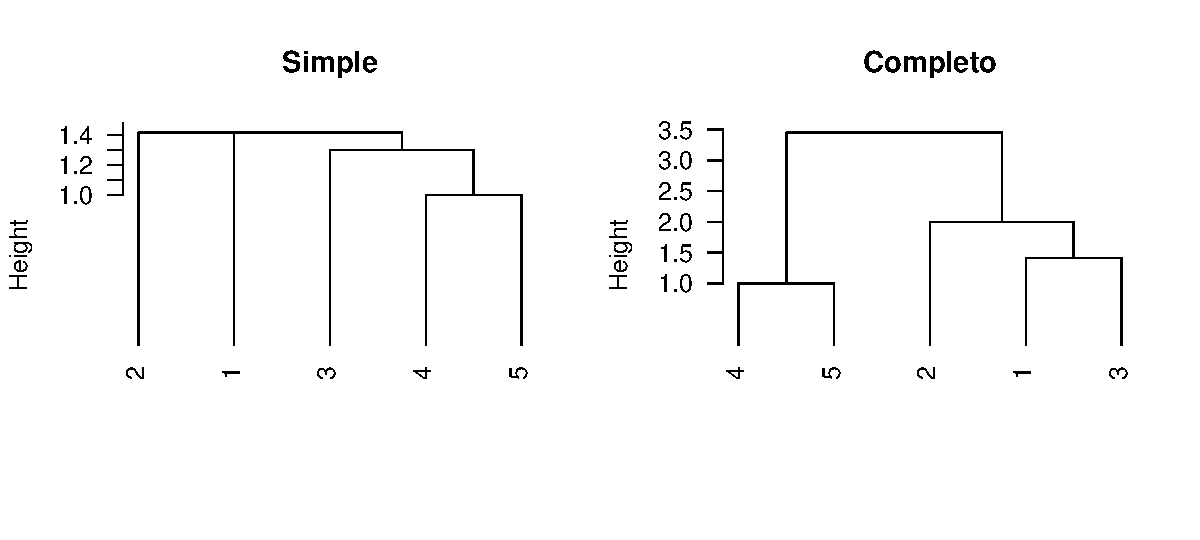
\includegraphics[width=0.9\textwidth]{figure/hc_toy_plot-1} 

}

\caption[Dendrogramas de los 5 puntos con enlace simple y completo]{Dendrogramas de los 5 puntos con enlace simple y completo.}\label{fig:hc_toy_plot}
\end{figure}

\end{knitrout}

%=====================================================================
\subsection{Combinación lineal de densidades}

Sea $f(x) = \sum_{j=1}^c \pi_j f_j(x\mid\theta_j)$ con $\pi_j\in[0,1]$, $\sum_{j=1}^c \pi_j = 1$ y cada $f_j$ una densidad en $\mathbb{R}^p$ (en el enunciado aparece $f_i$, lo tomo como $f_j$). Para que $f$ sea densidad necesito dos cosas:
\[
\text{(i) } f(x) \ge 0 \ \text{ para toda } x\in\mathbb{R}^p,
\qquad
\text{(ii) } \int_{\mathbb{R}^p} f(x)\,dx = 1.
\]

\textbf{(i) No negativa.} Para cualquier $x$ y cualquier $j$:
\[
\pi_j \ge 0 \quad\text{y}\quad f_j(x\mid\theta_j) \ge 0 \;\;(\text{porque } f_j \text{ es densidad})
\;\;\Longrightarrow\;\; \pi_j f_j(x\mid\theta_j) \ge 0.
\]
Una suma de términos no negativos es no negativa:
\[
f(x) = \sum_{j=1}^c \pi_j f_j(x\mid\theta_j) \ge 0.
\]

\textbf{(ii) Integra a uno.}
\begin{align*}
\int_{\mathbb{R}^p} f(x)\,dx
&= \int_{\mathbb{R}^p} \sum_{j=1}^c \pi_j f_j(x\mid\theta_j)\,dx\\
&= \sum_{j=1}^c \int_{\mathbb{R}^p} \pi_j f_j(x\mid\theta_j)\,dx
&& \text{(la integral de una suma finita es la suma de integrales)}\\
&= \sum_{j=1}^c \pi_j \int_{\mathbb{R}^p} f_j(x\mid\theta_j)\,dx
&& (\pi_j \text{ es constante, sale de la integral})\\
&= \sum_{j=1}^c \pi_j \cdot 1
&& (\text{cada } f_j \text{ es densidad})\\
&= \sum_{j=1}^c \pi_j\\
&= 1.
\end{align*}

Como se cumplen (i) y (ii), $f(x)$ es una función de densidad $p$-dimensional. \hfill$\square$

%=====================================================================
\subsection{Técnicas de clustering: votos republicanos 1960--1976}

\subsubsection*{Los datos}

\begin{knitrout}\small
\definecolor{shadecolor}{rgb}{0.969, 0.969, 0.969}\color{fgcolor}\begin{kframe}
\begin{alltt}
\hldef{votes} \hlkwb{<-} \hlkwd{read.table}\hldef{(}\hlsng{"../data/votes.txt"}\hldef{,} \hlkwc{check.names} \hldef{=} \hlnum{FALSE}\hldef{)}
\hlkwd{class}\hldef{(votes)}
\end{alltt}
\begin{verbatim}
[1] "data.frame"
\end{verbatim}
\begin{alltt}
\hlkwd{dim}\hldef{(votes)}
\end{alltt}
\begin{verbatim}
[1] 50  5
\end{verbatim}
\begin{alltt}
\hlkwd{names}\hldef{(votes)}
\end{alltt}
\begin{verbatim}
[1] "1960" "1964" "1968" "1972" "1976"
\end{verbatim}
\begin{alltt}
\hlkwd{head}\hldef{(votes)}
\end{alltt}
\begin{verbatim}
            1960 1964 1968 1972  1976
Alabama    41.75 69.5 14.0 72.4 43.48
Alaska     50.94 34.1 45.3 58.1 62.91
Arizona    55.52 50.4 54.8 64.7 58.62
Arkansas   43.06 43.9 30.8 68.9 34.97
California 50.10 40.9 47.8 55.0 50.89
Colorado   54.63 38.7 50.5 62.6 55.89
\end{verbatim}
\begin{alltt}
\hlkwd{round}\hldef{(}\hlkwd{sapply}\hldef{(votes, summary),} \hlnum{2}\hldef{)}
\end{alltt}
\begin{verbatim}
         1960  1964  1968  1972  1976
Min.    24.67 19.10 13.50 45.20 33.02
1st Qu. 48.58 34.88 40.58 58.52 46.90
Median  50.39 39.80 45.10 62.55 50.42
Mean    49.94 41.14 44.13 62.71 50.10
3rd Qu. 54.42 44.48 50.58 67.68 52.87
Max.    62.07 87.10 59.80 78.20 64.94
\end{verbatim}
\begin{alltt}
\hlkwd{round}\hldef{(}\hlkwd{cor}\hldef{(votes),} \hlnum{2}\hldef{)}
\end{alltt}
\begin{verbatim}
      1960  1964  1968  1972  1976
1960  1.00 -0.31  0.85 -0.08  0.54
1964 -0.31  1.00 -0.38  0.70 -0.03
1968  0.85 -0.38  1.00 -0.24  0.68
1972 -0.08  0.70 -0.24  1.00 -0.05
1976  0.54 -0.03  0.68 -0.05  1.00
\end{verbatim}
\end{kframe}
\end{knitrout}

\texttt{votes} es un \texttt{data.frame} con 50 filas y 5 columnas. Cada fila es un estado de EE.\,UU. y cada columna es el porcentaje de votos que obtuvo el candidato republicano a la presidencia en las elecciones de 1960, 1964, 1968, 1972 y 1976. Todas las variables están en la misma escala (porcentaje), así que trabajo con los datos sin estandarizar.

Algunas cosas que ya se ven desde aquí:
\begin{itemize}[leftmargin=*]
\item 1964 tiene la mayor dispersión (va de 19.1\% a 87.1\%) y 1972 tiene la media más alta (62.7\%).
\item 1960, 1968 y 1976 están correlacionadas positivamente entre sí ($0.85$ entre 1960 y 1968), mientras que 1964 y 1972 se correlacionan entre ellas ($0.70$) y van en sentido contrario al resto. Esto cuadra con que 1964 (Goldwater) y 1972 (McGovern) fueron años atípicos.
\end{itemize}

\begin{knitrout}\small
\definecolor{shadecolor}{rgb}{0.969, 0.969, 0.969}\color{fgcolor}\begin{kframe}
\begin{alltt}
\hlkwd{par}\hldef{(}\hlkwc{las} \hldef{=} \hlnum{1}\hldef{)}
\hlkwd{boxplot}\hldef{(votes,} \hlkwc{ylab} \hldef{=} \hlsng{"% voto republicano"}\hldef{,} \hlkwc{xlab} \hldef{=} \hlsng{"Elección"}\hldef{,} \hlkwc{col} \hldef{=} \hlsng{"grey90"}\hldef{)}
\end{alltt}
\end{kframe}\begin{figure}[H]

{\centering 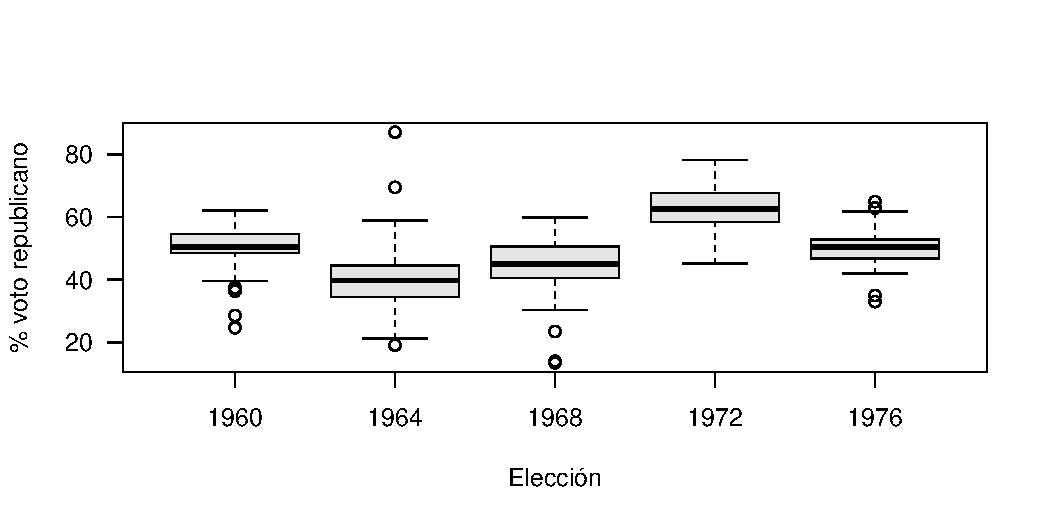
\includegraphics[width=0.75\textwidth]{figure/votes_box-1} 

}

\caption[Porcentaje de voto republicano por elección]{Porcentaje de voto republicano por elección.}\label{fig:votes_box}
\end{figure}

\end{knitrout}

%---------------------------------------------------------------------
\subsubsection*{Clustering jerárquico}

Sigo lo mismo que vimos en clase con \texttt{USArrests}: distancia euclidiana y los tres tipos de aglomeramiento.

\begin{knitrout}\small
\definecolor{shadecolor}{rgb}{0.969, 0.969, 0.969}\color{fgcolor}\begin{kframe}
\begin{alltt}
\hldef{D} \hlkwb{<-} \hlkwd{dist}\hldef{(votes,} \hlkwc{method} \hldef{=} \hlsng{"euclidean"}\hldef{)}
\hldef{xs} \hlkwb{<-} \hlkwd{hclust}\hldef{(D,} \hlsng{"single"}\hldef{)}
\hldef{xa} \hlkwb{<-} \hlkwd{hclust}\hldef{(D,} \hlsng{"average"}\hldef{)}
\hldef{xc} \hlkwb{<-} \hlkwd{hclust}\hldef{(D,} \hlsng{"complete"}\hldef{)}
\hldef{xl} \hlkwb{<-} \hlkwd{list}\hldef{(xs, xa, xc)}
\hldef{ml} \hlkwb{<-} \hlkwd{c}\hldef{(}\hlsng{"Single"}\hldef{,} \hlsng{"Average"}\hldef{,} \hlsng{"Complete"}\hldef{)}
\hlkwd{sapply}\hldef{(xl,} \hlkwa{function}\hldef{(}\hlkwc{h}\hldef{)} \hlkwd{round}\hldef{(}\hlkwd{rev}\hldef{(h}\hlopt{$}\hldef{height)[}\hlnum{1}\hlopt{:}\hlnum{5}\hldef{],} \hlnum{2}\hldef{))}
\end{alltt}
\begin{verbatim}
      [,1]  [,2]  [,3]
[1,] 25.85 51.31 76.58
[2,] 22.08 33.33 53.01
[3,] 20.56 30.28 45.77
[4,] 18.64 24.46 35.22
[5,] 13.74 22.08 34.71
\end{verbatim}
\begin{alltt}
\hlkwd{sapply}\hldef{(xl,} \hlkwa{function}\hldef{(}\hlkwc{h}\hldef{)} \hlkwd{table}\hldef{(}\hlkwd{cutree}\hldef{(h,} \hlkwc{k} \hldef{=} \hlnum{3}\hldef{)))}
\end{alltt}
\begin{verbatim}
  [,1] [,2] [,3]
1    1    3    3
2   48   45   37
3    1    2   10
\end{verbatim}
\end{kframe}
\end{knitrout}

\begin{knitrout}\small
\definecolor{shadecolor}{rgb}{0.969, 0.969, 0.969}\color{fgcolor}\begin{kframe}
\begin{alltt}
\hlkwd{par}\hldef{(}\hlkwc{mfrow} \hldef{=} \hlkwd{c}\hldef{(}\hlnum{3}\hldef{,} \hlnum{1}\hldef{),} \hlkwc{las} \hldef{=} \hlnum{1}\hldef{,} \hlkwc{mar} \hldef{=} \hlkwd{c}\hldef{(}\hlnum{1}\hldef{,} \hlnum{4}\hldef{,} \hlnum{3}\hldef{,} \hlnum{1}\hldef{))}
\hlkwa{for} \hldef{(i} \hlkwa{in} \hlnum{1}\hlopt{:}\hlnum{3}\hldef{) \{}
  \hlkwd{plot}\hldef{(xl[[i]],} \hlkwc{hang} \hldef{=} \hlopt{-}\hlnum{1}\hldef{,} \hlkwc{main} \hldef{= ml[i],} \hlkwc{sub} \hldef{=} \hlsng{""}\hldef{,} \hlkwc{xlab} \hldef{=} \hlsng{""}\hldef{,} \hlkwc{cex} \hldef{=} \hlnum{0.6}\hldef{)}
\hldef{\}}
\hlkwd{rect.hclust}\hldef{(xc,} \hlkwc{k} \hldef{=} \hlnum{3}\hldef{,} \hlkwc{border} \hldef{=} \hlnum{2}\hlopt{:}\hlnum{4}\hldef{)}
\end{alltt}
\end{kframe}\begin{figure}[H]

{\centering 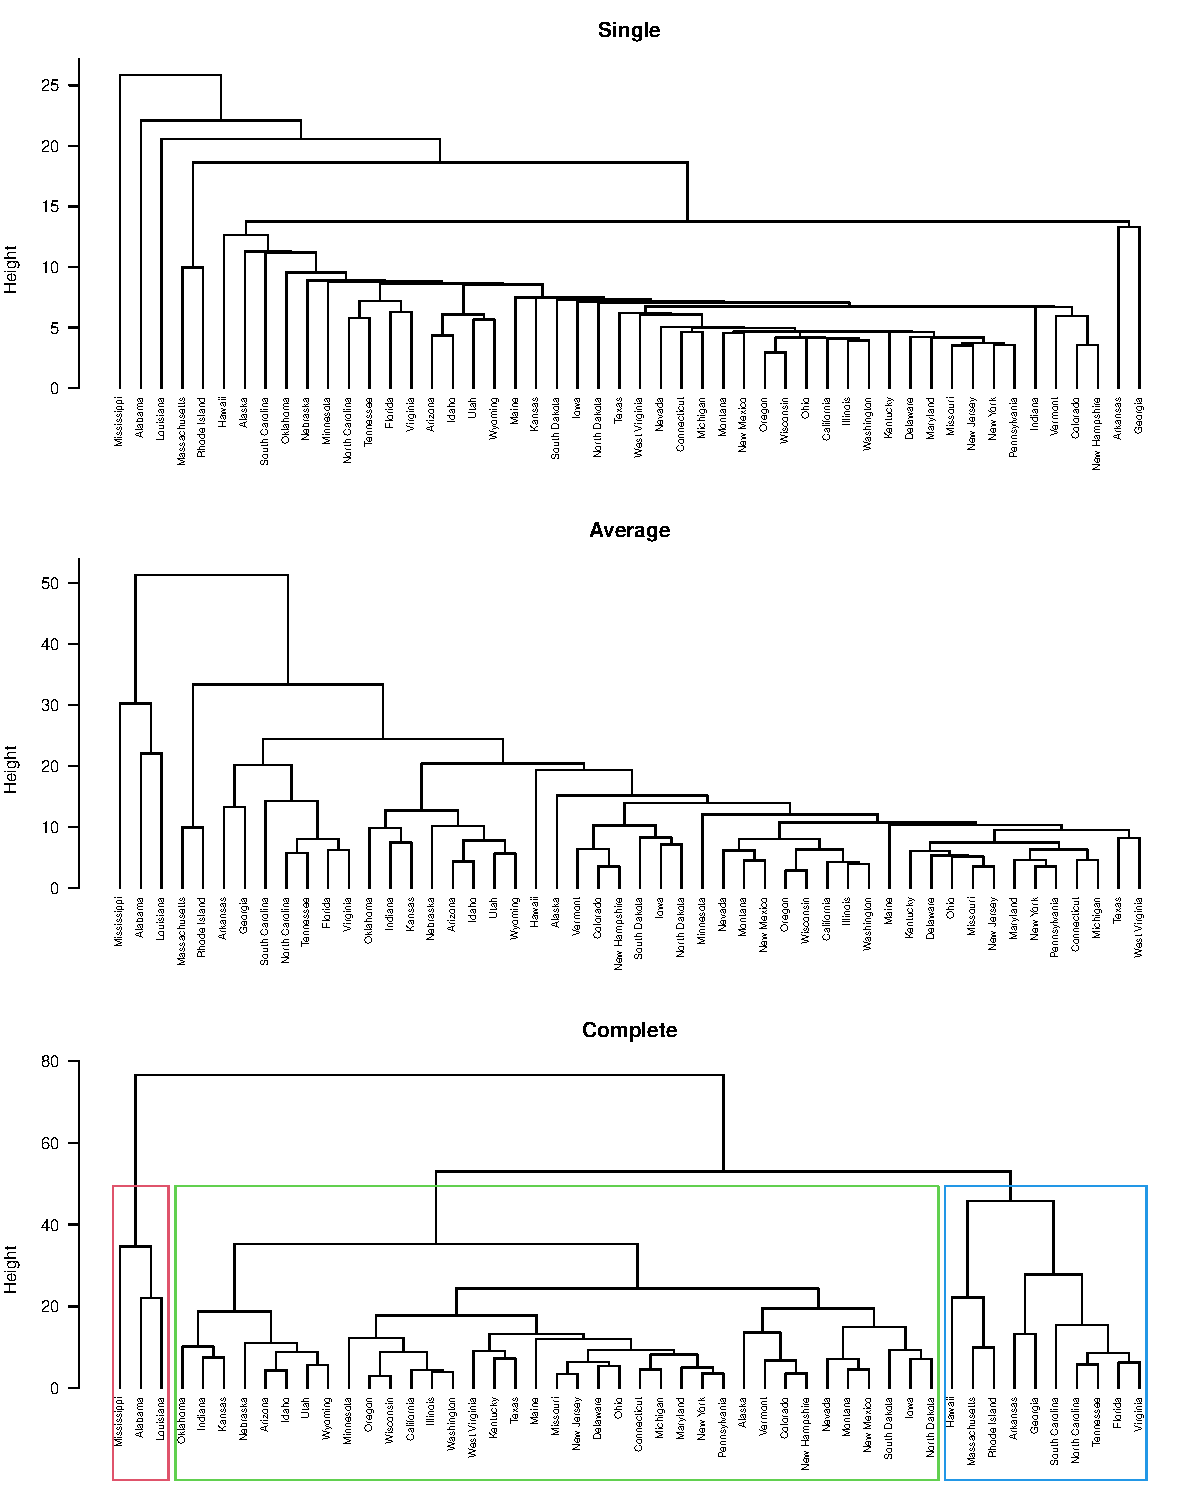
\includegraphics[width=\textwidth]{figure/votes_dend-1} 

}

\caption[Dendrogramas de los 50 estados]{Dendrogramas de los 50 estados. En el completo se marcan los 3 grupos.}\label{fig:votes_dend}
\end{figure}

\end{knitrout}

\begin{knitrout}\small
\definecolor{shadecolor}{rgb}{0.969, 0.969, 0.969}\color{fgcolor}\begin{kframe}
\begin{alltt}
\hldef{hcc} \hlkwb{<-} \hlkwd{cutree}\hldef{(xc,} \hlkwc{k} \hldef{=} \hlnum{3}\hldef{)}
\hlkwd{split}\hldef{(}\hlkwd{rownames}\hldef{(votes), hcc)}
\end{alltt}
\begin{verbatim}
$`1`
[1] "Alabama"     "Louisiana"   "Mississippi"

$`2`
 [1] "Alaska"        "Arizona"       "California"    "Colorado"     
 [5] "Connecticut"   "Delaware"      "Idaho"         "Illinois"     
 [9] "Indiana"       "Iowa"          "Kansas"        "Kentucky"     
[13] "Maine"         "Maryland"      "Michigan"      "Minnesota"    
[17] "Missouri"      "Montana"       "Nebraska"      "Nevada"       
[21] "New Hampshire" "New Jersey"    "New Mexico"    "New York"     
[25] "North Dakota"  "Ohio"          "Oklahoma"      "Oregon"       
[29] "Pennsylvania"  "South Dakota"  "Texas"         "Utah"         
[33] "Vermont"       "Washington"    "West Virginia" "Wisconsin"    
[37] "Wyoming"      

$`3`
 [1] "Arkansas"       "Florida"        "Georgia"        "Hawaii"        
 [5] "Massachusetts"  "North Carolina" "Rhode Island"   "South Carolina"
 [9] "Tennessee"      "Virginia"      
\end{verbatim}
\begin{alltt}
\hlkwd{round}\hldef{(}\hlkwd{aggregate}\hldef{(votes,} \hlkwc{by} \hldef{=} \hlkwd{list}\hldef{(}\hlkwc{cluster} \hldef{= hcc),} \hlkwc{FUN} \hldef{= mean),} \hlnum{2}\hldef{)}
\end{alltt}
\begin{verbatim}
  cluster  1960  1964  1968  1972  1976
1       1 31.67 71.13 17.00 71.97 46.56
2       2 52.49 38.88 48.47 61.27 52.27
3       3 45.99 40.47 36.19 65.23 43.16
\end{verbatim}
\begin{alltt}
\hlkwd{split}\hldef{(}\hlkwd{rownames}\hldef{(votes),} \hlkwd{cutree}\hldef{(xa,} \hlkwc{k} \hldef{=} \hlnum{3}\hldef{))}
\end{alltt}
\begin{verbatim}
$`1`
[1] "Alabama"     "Louisiana"   "Mississippi"

$`2`
 [1] "Alaska"         "Arizona"        "Arkansas"       "California"    
 [5] "Colorado"       "Connecticut"    "Delaware"       "Florida"       
 [9] "Georgia"        "Hawaii"         "Idaho"          "Illinois"      
[13] "Indiana"        "Iowa"           "Kansas"         "Kentucky"      
[17] "Maine"          "Maryland"       "Michigan"       "Minnesota"     
[21] "Missouri"       "Montana"        "Nebraska"       "Nevada"        
[25] "New Hampshire"  "New Jersey"     "New Mexico"     "New York"      
[29] "North Carolina" "North Dakota"   "Ohio"           "Oklahoma"      
[33] "Oregon"         "Pennsylvania"   "South Carolina" "South Dakota"  
[37] "Tennessee"      "Texas"          "Utah"           "Vermont"       
[41] "Virginia"       "Washington"     "West Virginia"  "Wisconsin"     
[45] "Wyoming"       

$`3`
[1] "Massachusetts" "Rhode Island" 
\end{verbatim}
\end{kframe}
\end{knitrout}

\textbf{Comentarios.}
\begin{itemize}[leftmargin=*]
\item \textbf{Simple:} sufre el efecto cadena; con $k=3$ solo separa a Alabama y a Mississippi como puntos sueltos y deja a los otros 48 juntos. No sirve mucho para interpretar.
\item \textbf{Promedio:} separa el grupo $\{$Alabama, Louisiana, Mississippi$\}$ y el par $\{$Massachusetts, Rhode Island$\}$, que son los estados menos republicanos en casi todos los años. El resto (45) queda junto.
\item \textbf{Completo:} es el más balanceado. Aísla otra vez $\{$Alabama, Louisiana, Mississippi$\}$, que votaron muy fuerte por Goldwater en 1964 y muy poco por Nixon en 1968. Un segundo grupo de 10 estados mezcla estados del sur (Georgia, Carolina del Sur, Arkansas, etc.) con Massachusetts, Rhode Island y Hawaii; lo que tienen en común es un voto republicano bajo en 1960 y 1968, aunque por razones muy distintas. El tercer grupo (37) es el resto del país.
\end{itemize}

%---------------------------------------------------------------------
\subsubsection*{$k$-medias}

Primero reviso cuántos grupos tomar con la suma de cuadrados dentro de grupos (TWSS), usando la función \texttt{f.twss} de clase.

\begin{knitrout}\small
\definecolor{shadecolor}{rgb}{0.969, 0.969, 0.969}\color{fgcolor}\begin{kframe}
\begin{alltt}
\hldef{f.twss} \hlkwb{<-} \hlkwa{function}\hldef{(}\hlkwc{X}\hldef{,} \hlkwc{k}\hldef{)\{}
  \hldef{twss} \hlkwb{<-} \hlkwd{sapply}\hldef{(k,} \hlkwa{function}\hldef{(}\hlkwc{k}\hldef{)} \hlkwd{kmeans}\hldef{(X, k,} \hlkwc{nstart} \hldef{=} \hlnum{100}\hldef{)}\hlopt{$}\hldef{tot.withinss)}
  \hlkwd{return}\hldef{(}\hlkwd{cbind}\hldef{(}\hlkwc{k} \hldef{= k,} \hlkwc{twss} \hldef{= twss))}
\hldef{\}}
\hlkwd{set.seed}\hldef{(}\hlnum{4}\hldef{)}
\hldef{twss} \hlkwb{<-} \hlkwd{f.twss}\hldef{(votes,} \hlnum{1}\hlopt{:}\hlnum{8}\hldef{)}
\hlkwd{round}\hldef{(twss,} \hlnum{1}\hldef{)}
\end{alltt}
\begin{verbatim}
     k    twss
[1,] 1 17445.9
[2,] 2  9978.3
[3,] 3  7129.2
[4,] 4  5381.9
[5,] 5  4238.0
[6,] 6  3585.6
[7,] 7  2964.0
[8,] 8  2566.7
\end{verbatim}
\begin{alltt}
\hlkwd{plot}\hldef{(twss,} \hlkwc{las} \hldef{=} \hlnum{1}\hldef{,} \hlkwc{type} \hldef{=} \hlsng{"b"}\hldef{,} \hlkwc{col} \hldef{=} \hlnum{4}\hldef{,} \hlkwc{bty} \hldef{=} \hlsng{"l"}\hldef{,} \hlkwc{pch} \hldef{=} \hlnum{19}\hldef{,}
     \hlkwc{xlab} \hldef{=} \hlsng{"Número de clusters k"}\hldef{,} \hlkwc{ylab} \hldef{=} \hlsng{"TWSS"}\hldef{)}
\hlkwd{abline}\hldef{(}\hlkwc{v} \hldef{=} \hlnum{3}\hldef{,} \hlkwc{lty} \hldef{=} \hlnum{2}\hldef{)}
\end{alltt}
\end{kframe}\begin{figure}[H]

{\centering 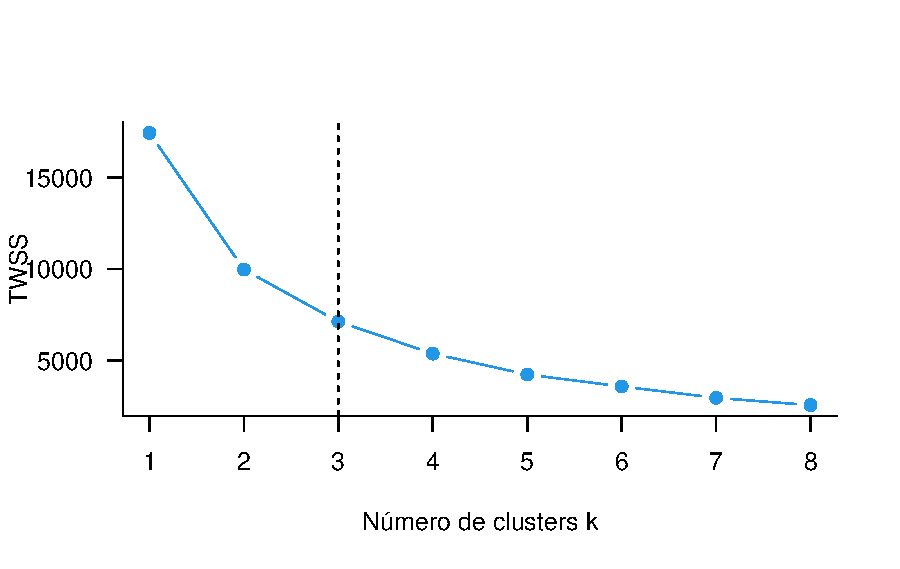
\includegraphics[width=0.6\textwidth]{figure/votes_twss-1} 

}

\caption[TWSS contra número de clusters]{TWSS contra número de clusters.}\label{fig:votes_twss}
\end{figure}

\end{knitrout}

La TWSS baja mucho de $k=1$ a $k=2$ y de $k=2$ a $k=3$; después las bajadas son cada vez más chicas. El ``codo'' está alrededor de $k=3$, que coincide con la sugerencia del ejercicio.

\begin{knitrout}\small
\definecolor{shadecolor}{rgb}{0.969, 0.969, 0.969}\color{fgcolor}\begin{kframe}
\begin{alltt}
\hlkwd{set.seed}\hldef{(}\hlnum{4}\hldef{)}
\hldef{km} \hlkwb{<-} \hlkwd{kmeans}\hldef{(votes,} \hlkwc{centers} \hldef{=} \hlnum{3}\hldef{,} \hlkwc{nstart} \hldef{=} \hlnum{100}\hldef{)}
\hldef{km}\hlopt{$}\hldef{size}
\end{alltt}
\begin{verbatim}
[1] 25  5 20
\end{verbatim}
\begin{alltt}
\hlkwd{round}\hldef{(km}\hlopt{$}\hldef{centers,} \hlnum{2}\hldef{)}
\end{alltt}
\begin{verbatim}
   1960  1964  1968  1972  1976
1 48.76 34.98 42.22 59.46 47.43
2 36.24 65.28 23.90 72.34 43.25
3 54.85 42.79 51.56 64.36 55.15
\end{verbatim}
\begin{alltt}
\hlkwd{split}\hldef{(}\hlkwd{rownames}\hldef{(votes), km}\hlopt{$}\hldef{cluster)}
\end{alltt}
\begin{verbatim}
$`1`
 [1] "Arkansas"       "California"     "Connecticut"    "Delaware"      
 [5] "Hawaii"         "Illinois"       "Kentucky"       "Maine"         
 [9] "Maryland"       "Massachusetts"  "Michigan"       "Minnesota"     
[13] "Missouri"       "New Jersey"     "New York"       "North Carolina"
[17] "Ohio"           "Oregon"         "Pennsylvania"   "Rhode Island"  
[21] "Tennessee"      "Texas"          "Washington"     "West Virginia" 
[25] "Wisconsin"     

$`2`
[1] "Alabama"        "Georgia"        "Louisiana"      "Mississippi"   
[5] "South Carolina"

$`3`
 [1] "Alaska"        "Arizona"       "Colorado"      "Florida"      
 [5] "Idaho"         "Indiana"       "Iowa"          "Kansas"       
 [9] "Montana"       "Nebraska"      "Nevada"        "New Hampshire"
[13] "New Mexico"    "North Dakota"  "Oklahoma"      "South Dakota" 
[17] "Utah"          "Vermont"       "Virginia"      "Wyoming"      
\end{verbatim}
\begin{alltt}
\hlkwd{round}\hldef{(}\hlkwd{c}\hldef{(}\hlkwc{between} \hldef{= km}\hlopt{$}\hldef{betweenss,} \hlkwc{within} \hldef{= km}\hlopt{$}\hldef{tot.withinss,} \hlkwc{total} \hldef{= km}\hlopt{$}\hldef{totss,}
        \hlkwc{ratio} \hldef{= km}\hlopt{$}\hldef{betweenss} \hlopt{/} \hldef{km}\hlopt{$}\hldef{totss),} \hlnum{3}\hldef{)}
\end{alltt}
\begin{verbatim}
  between    within     total     ratio 
10316.730  7129.178 17445.909     0.591 
\end{verbatim}
\end{kframe}
\end{knitrout}

También lo comparo con la función \texttt{my.km} que hicimos en clase:

\begin{knitrout}\small
\definecolor{shadecolor}{rgb}{0.969, 0.969, 0.969}\color{fgcolor}\begin{kframe}
\begin{alltt}
\hlkwd{source}\hldef{(}\hlsng{"../rcode/my_kmeans.R"}\hldef{)}
\hlkwd{set.seed}\hldef{(}\hlnum{4}\hldef{)}
\hldef{a} \hlkwb{<-} \hlkwd{my.km}\hldef{(votes,} \hlnum{3}\hldef{)}
\hlkwd{table}\hldef{(}\hlkwc{my.km} \hldef{= a}\hlopt{$}\hldef{cluster,} \hlkwc{kmeans} \hldef{= km}\hlopt{$}\hldef{cluster)}
\end{alltt}
\begin{verbatim}
     kmeans
my.km  1  2  3
    1  3  0  0
    2  1  5  0
    3 21  0 20
\end{verbatim}
\begin{alltt}
\hlkwd{rbind}\hldef{(}\hlkwc{my.km} \hldef{=} \hlkwd{unlist}\hldef{(a[}\hlkwd{c}\hldef{(}\hlsng{"between.ss"}\hldef{,} \hlsng{"twithin.ss"}\hldef{,} \hlsng{"total.ss"}\hldef{)]),}
      \hlkwc{kmeans} \hldef{=} \hlkwd{c}\hldef{(km}\hlopt{$}\hldef{betweenss, km}\hlopt{$}\hldef{tot.withinss, km}\hlopt{$}\hldef{totss))}
\end{alltt}
\begin{verbatim}
       between.ss twithin.ss total.ss
my.km    9507.983   7937.925 17445.91
kmeans  10316.730   7129.178 17445.91
\end{verbatim}
\end{kframe}
\end{knitrout}

Con un solo arranque aleatorio, \texttt{my.km} se queda en una solución peor (TWSS de 7937.9 contra 7129.2): junta casi todo en un grupo grande y deja uno de solo 3 estados. Por eso es importante usar \texttt{nstart = 100} en \texttt{kmeans}, que prueba muchos arranques y se queda con el mejor. De aquí en adelante uso el resultado de \texttt{kmeans}.

\begin{knitrout}\small
\definecolor{shadecolor}{rgb}{0.969, 0.969, 0.969}\color{fgcolor}\begin{kframe}
\begin{alltt}
\hldef{yrs} \hlkwb{<-} \hlkwd{as.numeric}\hldef{(}\hlkwd{names}\hldef{(votes))}
\hlkwd{matplot}\hldef{(yrs,} \hlkwd{t}\hldef{(km}\hlopt{$}\hldef{centers),} \hlkwc{type} \hldef{=} \hlsng{"b"}\hldef{,} \hlkwc{pch} \hldef{=} \hlnum{19}\hldef{,} \hlkwc{lty} \hldef{=} \hlnum{1}\hldef{,} \hlkwc{col} \hldef{=} \hlnum{1}\hlopt{:}\hlnum{3}\hldef{,}
        \hlkwc{las} \hldef{=} \hlnum{1}\hldef{,} \hlkwc{xaxt} \hldef{=} \hlsng{"n"}\hldef{,} \hlkwc{xlab} \hldef{=} \hlsng{"Elección"}\hldef{,} \hlkwc{ylab} \hldef{=} \hlsng{"% voto republicano"}\hldef{)}
\hlkwd{axis}\hldef{(}\hlnum{1}\hldef{,} \hlkwc{at} \hldef{= yrs)}
\hlkwd{legend}\hldef{(}\hlsng{"topleft"}\hldef{,} \hlkwc{legend} \hldef{=} \hlkwd{paste}\hldef{(}\hlsng{"Cluster"}\hldef{,} \hlnum{1}\hlopt{:}\hlnum{3}\hldef{,} \hlsng{"( n ="}\hldef{, km}\hlopt{$}\hldef{size,} \hlsng{")"}\hldef{),}
       \hlkwc{col} \hldef{=} \hlnum{1}\hlopt{:}\hlnum{3}\hldef{,} \hlkwc{lty} \hldef{=} \hlnum{1}\hldef{,} \hlkwc{pch} \hldef{=} \hlnum{19}\hldef{,} \hlkwc{bty} \hldef{=} \hlsng{"n"}\hldef{)}
\end{alltt}
\end{kframe}\begin{figure}[H]

{\centering 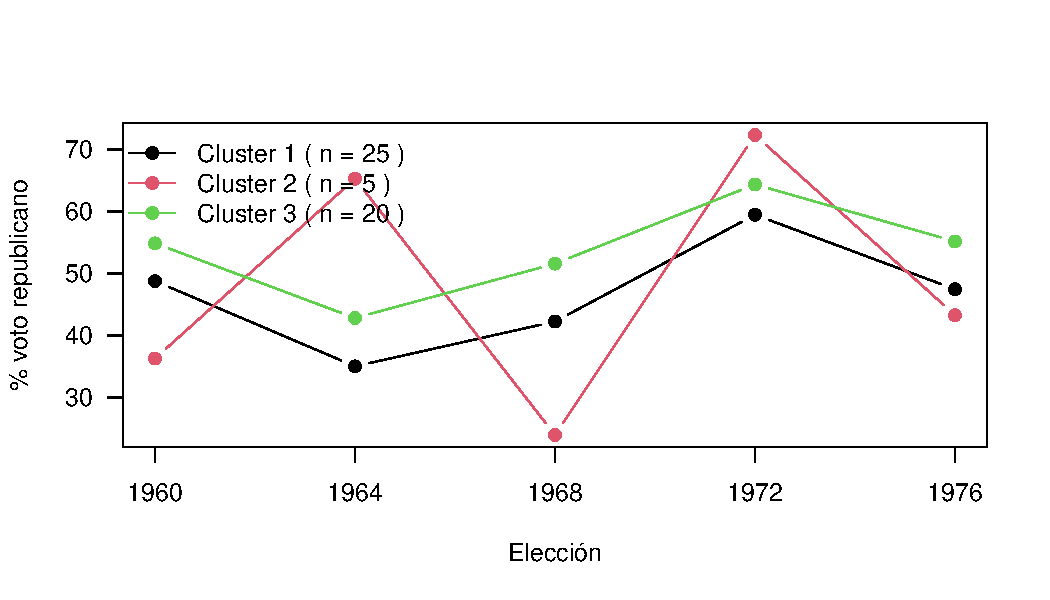
\includegraphics[width=0.75\textwidth]{figure/votes_km_prof-1} 

}

\caption[Centros de k-medias (k=3) a lo largo de las elecciones]{Centros de k-medias (k=3) a lo largo de las elecciones.}\label{fig:votes_km_prof}
\end{figure}

\end{knitrout}

\textbf{Comentarios.} Con $k=3$ los grupos se pueden leer fácil:
\begin{itemize}[leftmargin=*]
\item \textbf{Cluster 2 (sur profundo, 5 estados):} Alabama, Georgia, Louisiana, Mississippi y Carolina del Sur. Voto republicano bajo en 1960, muy alto en 1964 (Goldwater, alrededor del 65\%), muy bajo en 1968 (en ese año gran parte del voto del sur se fue a un tercer candidato), y otra vez alto en 1972. Es el grupo con el patrón más ``brincado''.
\item \textbf{Cluster 3 (más republicanos, 20 estados):} sobre todo estados del oeste y de las planicies (Arizona, Colorado, Idaho, Kansas, Nebraska, Utah, Wyoming, etc.) más algunos como Florida, Indiana, Oklahoma y Virginia. Votan más por el republicano que el promedio en casi todas las elecciones.
\item \textbf{Cluster 1 (menos republicanos, 25 estados):} noreste, medio oeste industrial y la costa del Pacífico (Nueva York, Massachusetts, Illinois, Michigan, California, Washington, etc.) más algunos estados del sur y fronterizos (Arkansas, Kentucky, Tennessee, Texas, West Virginia). Siguen el mismo patrón que el grupo anterior pero siempre unos puntos abajo.
\end{itemize}
Los dos grupos grandes se mueven en paralelo de una elección a otra (sube y baja el ánimo nacional), y lo que los separa es básicamente el nivel. El grupo pequeño se separa por la forma del patrón, en especial por 1964 y 1968. La razón $\text{BSS}/\text{TSS}$ de 0.59 dice que los 3 grupos explican cerca del 59\% de la variabilidad total.

%---------------------------------------------------------------------
\subsubsection*{Mixtura de densidades (\texttt{Mclust})}

Primero dejo que \texttt{Mclust} escoja el modelo y el número de componentes con el BIC.

\begin{knitrout}\small
\definecolor{shadecolor}{rgb}{0.969, 0.969, 0.969}\color{fgcolor}\begin{kframe}
\begin{alltt}
\hlkwd{library}\hldef{(mclust)}
\hldef{mc} \hlkwb{<-} \hlkwd{Mclust}\hldef{(votes)}
\hlkwd{summary}\hldef{(mc)}
\end{alltt}
\begin{verbatim}
---------------------------------------------------- 
Gaussian finite mixture model fitted by EM algorithm 
---------------------------------------------------- 

Mclust VVE (ellipsoidal, equal orientation) model with 2 components: 

 log-likelihood  n df       BIC       ICL
      -734.7031 50 31 -1590.679 -1594.198

Clustering table:
 1  2 
17 33 
\end{verbatim}
\begin{alltt}
\hlkwd{split}\hldef{(}\hlkwd{rownames}\hldef{(votes), mc}\hlopt{$}\hldef{classification)}
\end{alltt}
\begin{verbatim}
$`1`
 [1] "Alabama"        "Alaska"         "Arkansas"       "Florida"       
 [5] "Georgia"        "Kentucky"       "Louisiana"      "Maine"         
 [9] "Mississippi"    "North Carolina" "Oklahoma"       "South Carolina"
[13] "Tennessee"      "Texas"          "Vermont"        "Virginia"      
[17] "West Virginia" 

$`2`
 [1] "Arizona"       "California"    "Colorado"      "Connecticut"  
 [5] "Delaware"      "Hawaii"        "Idaho"         "Illinois"     
 [9] "Indiana"       "Iowa"          "Kansas"        "Maryland"     
[13] "Massachusetts" "Michigan"      "Minnesota"     "Missouri"     
[17] "Montana"       "Nebraska"      "Nevada"        "New Hampshire"
[21] "New Jersey"    "New Mexico"    "New York"      "North Dakota" 
[25] "Ohio"          "Oregon"        "Pennsylvania"  "Rhode Island" 
[29] "South Dakota"  "Utah"          "Washington"    "Wisconsin"    
[33] "Wyoming"      
\end{verbatim}
\end{kframe}
\end{knitrout}

\begin{knitrout}\small
\definecolor{shadecolor}{rgb}{0.969, 0.969, 0.969}\color{fgcolor}\begin{kframe}
\begin{alltt}
\hlkwd{plot}\hldef{(mc,} \hlkwc{what} \hldef{=} \hlsng{"BIC"}\hldef{)}
\end{alltt}
\end{kframe}\begin{figure}[H]

{\centering 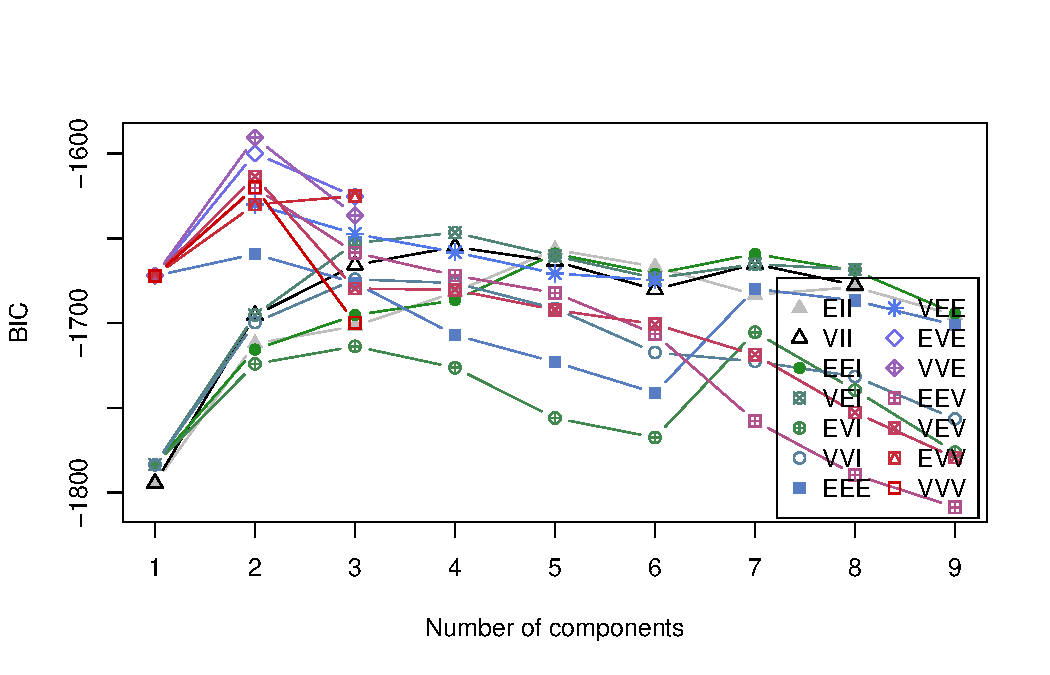
\includegraphics[width=0.7\textwidth]{figure/votes_bic-1} 

}

\caption[BIC de los modelos de mixtura]{BIC de los modelos de mixtura.}\label{fig:votes_bic}
\end{figure}

\end{knitrout}

Para compararlo con $k$-medias también ajusto con 3 componentes:

\begin{knitrout}\small
\definecolor{shadecolor}{rgb}{0.969, 0.969, 0.969}\color{fgcolor}\begin{kframe}
\begin{alltt}
\hldef{mc3} \hlkwb{<-} \hlkwd{Mclust}\hldef{(votes,} \hlkwc{G} \hldef{=} \hlnum{3}\hldef{)}
\hlkwd{summary}\hldef{(mc3)}
\end{alltt}
\begin{verbatim}
---------------------------------------------------- 
Gaussian finite mixture model fitted by EM algorithm 
---------------------------------------------------- 

Mclust EVV (ellipsoidal, equal volume) model with 3 components: 

 log-likelihood  n df       BIC       ICL
      -695.1362 50 60 -1624.994 -1630.003

Clustering table:
 1  2  3 
 8 25 17 
\end{verbatim}
\begin{alltt}
\hlkwd{round}\hldef{(mc3}\hlopt{$}\hldef{parameters}\hlopt{$}\hldef{pro,} \hlnum{3}\hldef{)}
\end{alltt}
\begin{verbatim}
[1] 0.160 0.535 0.305
\end{verbatim}
\begin{alltt}
\hlkwd{round}\hldef{(}\hlkwd{t}\hldef{(mc3}\hlopt{$}\hldef{parameters}\hlopt{$}\hldef{mean),} \hlnum{2}\hldef{)}
\end{alltt}
\begin{verbatim}
      1960  1964  1968  1972  1976
[1,] 40.19 52.69 29.70 68.87 44.62
[2,] 50.25 35.73 45.83 58.24 49.86
[3,] 54.51 44.56 48.68 67.31 53.40
\end{verbatim}
\begin{alltt}
\hlkwd{split}\hldef{(}\hlkwd{rownames}\hldef{(votes), mc3}\hlopt{$}\hldef{classification)}
\end{alltt}
\begin{verbatim}
$`1`
[1] "Alabama"        "Alaska"         "Arkansas"       "Georgia"       
[5] "Louisiana"      "Mississippi"    "North Carolina" "West Virginia" 

$`2`
 [1] "California"    "Connecticut"   "Delaware"      "Hawaii"       
 [5] "Illinois"      "Iowa"          "Maine"         "Maryland"     
 [9] "Massachusetts" "Michigan"      "Minnesota"     "Missouri"     
[13] "Montana"       "Nevada"        "New Jersey"    "New Mexico"   
[17] "New York"      "North Dakota"  "Ohio"          "Oregon"       
[21] "Pennsylvania"  "Rhode Island"  "South Dakota"  "Washington"   
[25] "Wisconsin"    

$`3`
 [1] "Arizona"        "Colorado"       "Florida"        "Idaho"         
 [5] "Indiana"        "Kansas"         "Kentucky"       "Nebraska"      
 [9] "New Hampshire"  "Oklahoma"       "South Carolina" "Tennessee"     
[13] "Texas"          "Utah"           "Vermont"        "Virginia"      
[17] "Wyoming"       
\end{verbatim}
\begin{alltt}
\hlkwd{round}\hldef{(}\hlkwd{sort}\hldef{(mc3}\hlopt{$}\hldef{uncertainty,} \hlkwc{decreasing} \hldef{=} \hlnum{TRUE}\hldef{)[}\hlnum{1}\hlopt{:}\hlnum{6}\hldef{],} \hlnum{3}\hldef{)}
\end{alltt}
\begin{verbatim}
New Hampshire        Kansas      Colorado      Kentucky       Indiana 
        0.483         0.466         0.386         0.199         0.111 
      Vermont 
        0.078 
\end{verbatim}
\end{kframe}
\end{knitrout}

\textbf{Comentarios.}
\begin{itemize}[leftmargin=*]
\item Según el BIC el mejor modelo es \texttt{VVE} con 2 componentes. Hay que tomar en cuenta que con solo 50 estados y 5 variables, los modelos con covarianzas libres tienen muchos parámetros, y el BIC castiga eso; por eso prefiere pocos grupos.
\item Con 2 componentes la separación es, a grandes rasgos, sur y estados fronterizos (más algunos como Alaska, Maine y Vermont) contra el resto del país. No es la división por nivel que da $k$-medias, sino una división más ligada a la forma de las covarianzas.
\item Con 3 componentes (\texttt{EVV}) aparece otra vez un grupo del sur, aunque más amplio que en $k$-medias (agrega Arkansas, Carolina del Norte, Alaska y West Virginia y saca a Carolina del Sur), un grupo grande de noreste, medio oeste y Pacífico, y un grupo del oeste y planicies con algunos estados del sur.
\item A diferencia de $k$-medias, \texttt{Mclust} da probabilidades de pertenencia. Los estados con mayor incertidumbre son los que quedan ``en la frontera'' entre grupos.
\end{itemize}

%---------------------------------------------------------------------
\subsubsection*{Comparación de los métodos}

\begin{knitrout}\small
\definecolor{shadecolor}{rgb}{0.969, 0.969, 0.969}\color{fgcolor}\begin{kframe}
\begin{alltt}
\hlkwd{table}\hldef{(}\hlkwc{hclust} \hldef{= hcc,} \hlkwc{kmeans} \hldef{= km}\hlopt{$}\hldef{cluster)}
\end{alltt}
\begin{verbatim}
      kmeans
hclust  1  2  3
     1  0  3  0
     2 19  0 18
     3  6  2  2
\end{verbatim}
\begin{alltt}
\hlkwd{table}\hldef{(}\hlkwc{kmeans} \hldef{= km}\hlopt{$}\hldef{cluster,} \hlkwc{mclust3} \hldef{= mc3}\hlopt{$}\hldef{classification)}
\end{alltt}
\begin{verbatim}
      mclust3
kmeans  1  2  3
     1  3 19  3
     2  4  0  1
     3  1  6 13
\end{verbatim}
\begin{alltt}
\hlkwd{table}\hldef{(}\hlkwc{kmeans} \hldef{= km}\hlopt{$}\hldef{cluster,} \hlkwc{mclust} \hldef{= mc}\hlopt{$}\hldef{classification)}
\end{alltt}
\begin{verbatim}
      mclust
kmeans  1  2
     1  7 18
     2  5  0
     3  5 15
\end{verbatim}
\begin{alltt}
\hlkwd{round}\hldef{(}\hlkwd{c}\hldef{(}\hlkwc{hc_km} \hldef{=} \hlkwd{adjustedRandIndex}\hldef{(hcc, km}\hlopt{$}\hldef{cluster),}
        \hlkwc{km_mc3} \hldef{=} \hlkwd{adjustedRandIndex}\hldef{(km}\hlopt{$}\hldef{cluster, mc3}\hlopt{$}\hldef{classification),}
        \hlkwc{hc_mc3} \hldef{=} \hlkwd{adjustedRandIndex}\hldef{(hcc, mc3}\hlopt{$}\hldef{classification)),} \hlnum{3}\hldef{)}
\end{alltt}
\begin{verbatim}
 hc_km km_mc3 hc_mc3 
 0.167  0.296  0.171 
\end{verbatim}
\end{kframe}
\end{knitrout}

\begin{knitrout}\small
\definecolor{shadecolor}{rgb}{0.969, 0.969, 0.969}\color{fgcolor}\begin{kframe}
\begin{alltt}
\hldef{uprplt} \hlkwb{<-} \hlkwa{function}\hldef{(}\hlkwc{x}\hldef{,} \hlkwc{y}\hldef{) \{}\hlkwd{points}\hldef{(x, y,} \hlkwc{col} \hldef{= km}\hlopt{$}\hldef{cluster,} \hlkwc{pch} \hldef{= km}\hlopt{$}\hldef{cluster)\}}
\hldef{lwrplt} \hlkwb{<-} \hlkwa{function}\hldef{(}\hlkwc{x}\hldef{,} \hlkwc{y}\hldef{) \{}\hlkwd{points}\hldef{(x, y,} \hlkwc{col} \hldef{= mc3}\hlopt{$}\hldef{classification,} \hlkwc{pch} \hldef{= mc3}\hlopt{$}\hldef{classification)\}}
\hlkwd{pairs}\hldef{(votes,} \hlkwc{lower.panel} \hldef{= lwrplt,} \hlkwc{upper.panel} \hldef{= uprplt)}
\end{alltt}
\end{kframe}\begin{figure}[H]

{\centering 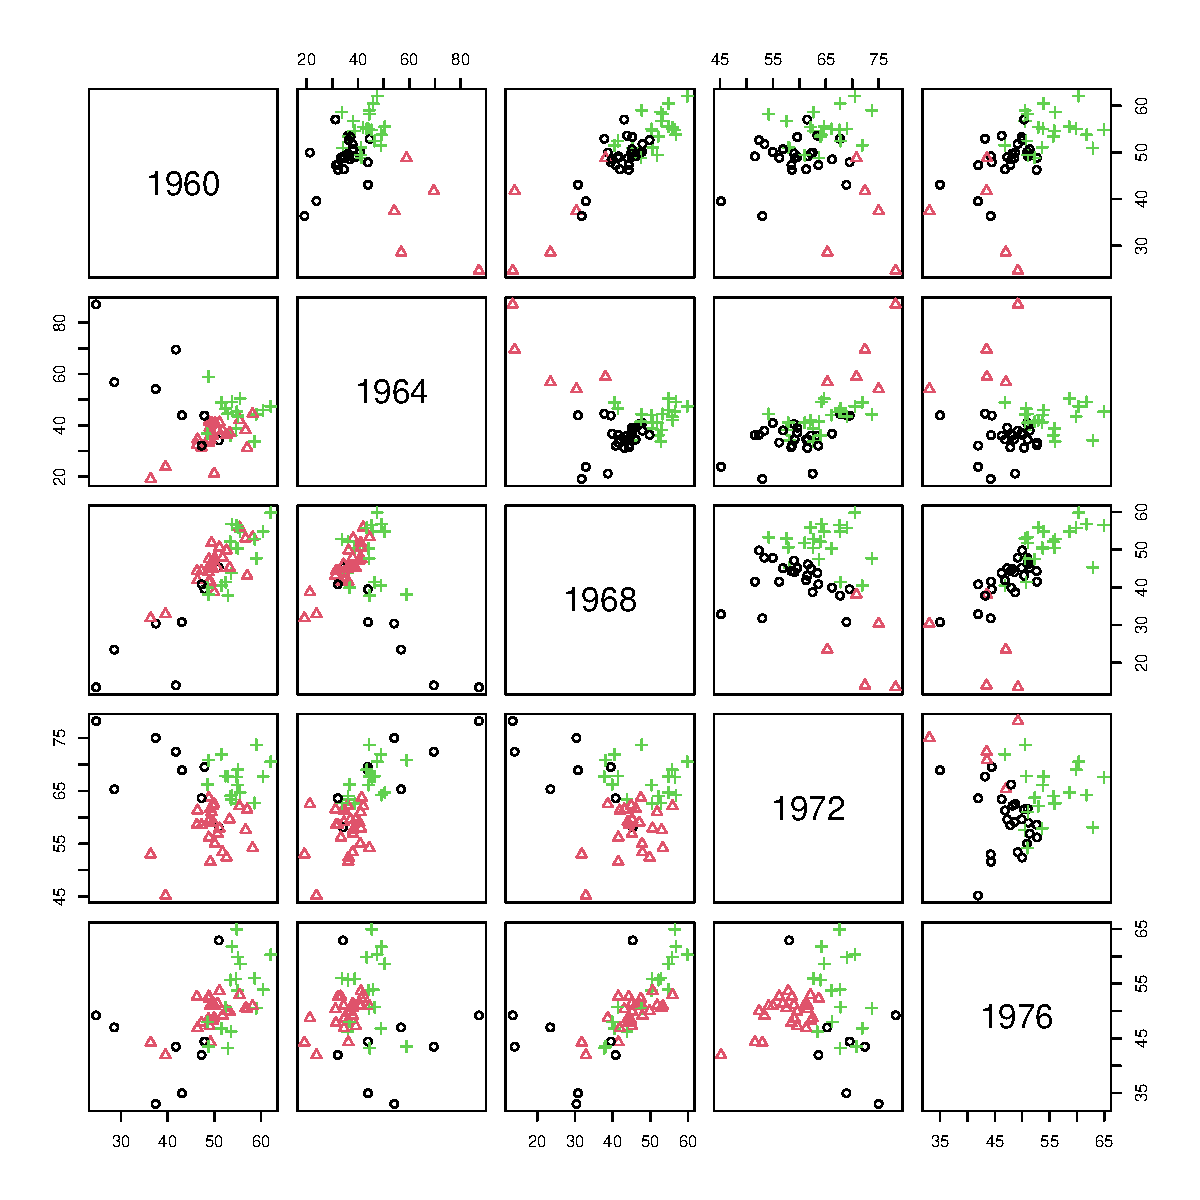
\includegraphics[width=0.85\textwidth]{figure/votes_pairs-1} 

}

\caption[Arriba de la diagonal]{Arriba de la diagonal: k-medias (k=3). Abajo: Mclust con 3 componentes.}\label{fig:votes_pairs}
\end{figure}

\end{knitrout}

\textbf{Interpretación general.}
\begin{itemize}[leftmargin=*]
\item \textbf{Lo que todos encuentran:} un núcleo del sur profundo (Alabama, Louisiana, Mississippi, y casi siempre Georgia y Carolina del Sur) con un patrón muy distinto al resto: mucho voto republicano en 1964, poco en 1960 y 1968. Esto es justo lo que se espera por la candidatura de Goldwater en 1964. En 1972 casi todo el país votó republicano (McGovern), así que ese año ayuda poco a separar grupos, salvo que el sur llegó a los niveles más altos.
\item \textbf{Jerárquico:} depende mucho del tipo de enlace. El simple no sirve aquí por el efecto cadena; el completo da algo interpretable, pero su segundo grupo mezcla estados que coinciden en tener voto bajo en 1960 y 1968 aunque por razones muy distintas (el sur y Massachusetts/Rhode Island). Además, una vez que une dos estados ya no los puede separar.
\item \textbf{$k$-medias con $k=3$:} es la lectura más clara: sur profundo, estados más republicanos (oeste y planicies) y estados menos republicanos (noreste, medio oeste industrial, Pacífico). Los dos grupos grandes se distinguen por el nivel y el pequeño por la forma del patrón. La desventaja es que asume grupos más o menos esféricos y del mismo tamaño.
\item \textbf{Mixtura de densidades:} permite grupos con distinta forma y tamaño y da una medida de incertidumbre, lo cual es útil para los estados en la frontera. Pero con tan pocos datos el BIC se queda con 2 componentes y los grupos son menos fáciles de explicar que los de $k$-medias. Con 3 componentes se parece más a $k$-medias, sobre todo en el grupo del sur.
\item Las tablas y el índice de Rand ajustado (valores entre 0.17 y 0.30) muestran que el acuerdo entre métodos es bajo a moderado. Coinciden en el grupo atípico del sur, pero reparten de forma distinta a los estados ``del medio''. Por ejemplo, el grupo grande de 37 estados del completo se parte casi a la mitad en $k$-medias (19 y 18), es decir, el completo no separa por nivel de voto como sí lo hace $k$-medias.
\end{itemize}

En resumen, para estos datos me quedo con $k$-medias con $k=3$ como la partición más fácil de interpretar, y uso el completo y \texttt{Mclust} para confirmar que el grupo del sur es real y no un resultado de un solo método.

\end{document}
